\chapter{The Normal Distribution}

\section{Density/Distribution Curve }
A density/distribution curve is a smoothed histogram. Examples of density/distribution curves are below.

\begin{figure}[h!]
\centering
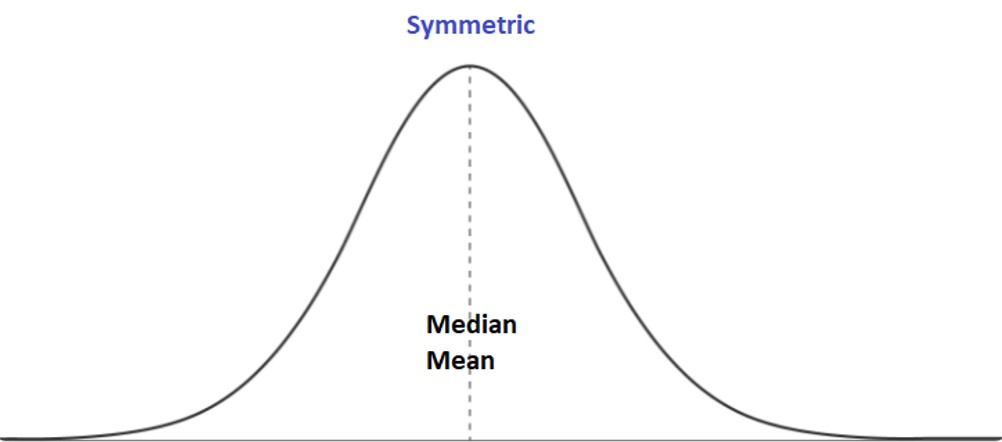
\includegraphics[width=0.6\textwidth]{figures/ch3.1a.jpg}
\caption{In a symmetric distribution the Mean and Median are the same.}
\label{fig:ch3.1a.jpg}
\end{figure}

\begin{figure}[h!]
\centering
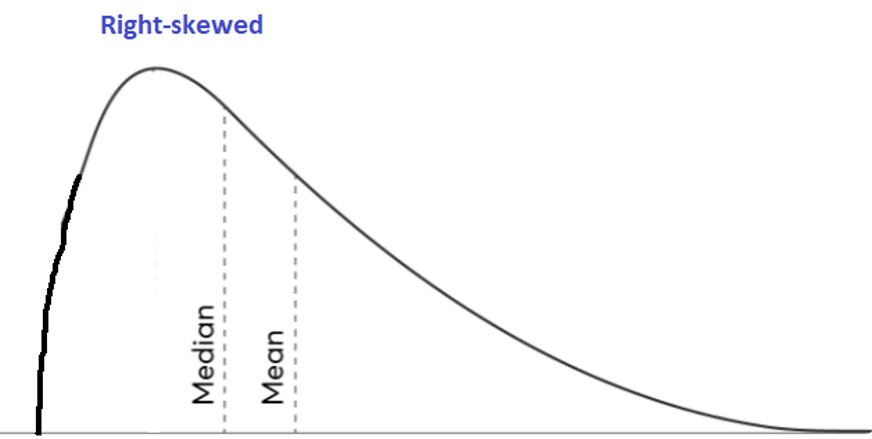
\includegraphics[width=0.6\textwidth]{figures/ch3.1b.jpg}
\caption{Notice that the density curve has a tail to the right. In a right-skewed distribution the Mean is greater than the Median (M).}
\label{fig:ch3.1b.jpg}
\end{figure}

\begin{figure}[h!]
\centering
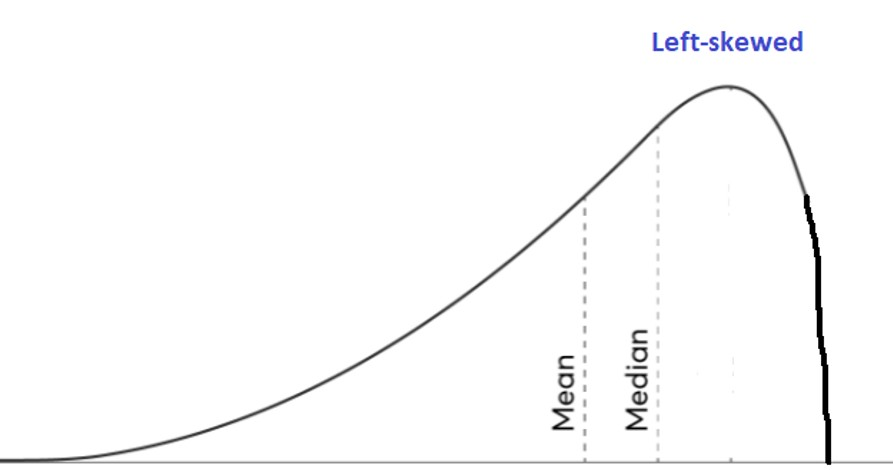
\includegraphics[width=0.6\textwidth]{figures/ch3.1c.jpg}
\caption{Notice that the density curve has a tail to the left. In a left-skewed distribution the Mean is less than the Median (M).}
\label{fig:ch3.1c.jpg}
\end{figure}

\vspace{0.5cm}

The following are properties of a density curve:
\begin{enumerate}
    \item The total area under a density curve is 1.
    \item The area under the density curve and above any range of values is the proportion of all observations that fall in that range.
\end{enumerate}


\section{Normal Distribution}
A Normal distribution is completely described by its mean $\mu$ and standard deviation $\sigma$. We represent a Normal distribution as \(N(\mu, \sigma).\) Figure \ref{fig:normal_density.jpg} is an example of a normal distribution curve.

A Normal distribution curve has the following properties:
\begin{enumerate}
    \item Symmetric, single-peaked, bell-shaped.
    \item Completely described by giving its mean $\mu$ and its standard deviation $\sigma$.
    \item Mean and median are located at the center (they are the same).
    \item Standard deviation controls variability: bigger standard deviation implies wider curve.
\end{enumerate}

\textbf{Note:} The standard deviation of the normal distribution is the distance from the center to the change-of-curvature points on either side.


\subsection{The 68-95-99.7 Rule }
In the Normal distribution with mean $\mu$ and standard deviation $\sigma$:

\begin{itemize}
    \item Approximately 68\% of the observations fall within $\sigma$ of the mean $\mu$.
    \item Approximately 95\% of the observations fall within $2\sigma$ of $\mu$.
    \item Approximately 99.7\% of the observations fall within $3\sigma$ of $\mu$.
\end{itemize}

\begin{figure}[h!]
\centering
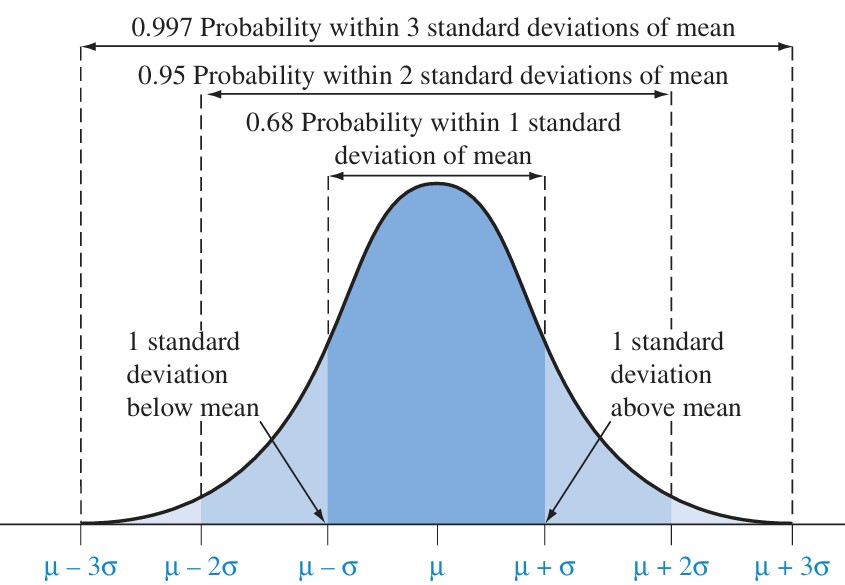
\includegraphics[width=0.6\textwidth]{figures/normal_density.jpg}
\caption{The Normal Distribution Curve}
\label{fig:normal_density.jpg}
\end{figure}

\subsubsection*{Example 1 about the Normal Distribution}
The test scores of UGA statistics students are graded on a 10-point scale. These scores are Normally distributed with a mean $\mu = 6.84$ and a standard deviation $\sigma = 1.55$. What range of scores has 95\% of the student scores?

\textbf{Solution}
\[
\mu - 2\sigma = 6.84 - 2(1.55) = 6.84 - 3.10 = 3.74
\]
\[
\mu + 2\sigma = 6.84 + 2(1.55) = 6.84 + 3.10 = 9.94
\]

Therefore, 95\% of the students scored between 3.74 and 9.94.

\section{Standard Normal Distribution}
A Standard Normal distribution is a type of normal distribution with a mean of 0 and a standard deviation of 1. So, for a Standard Normal distribution we have: \(N(0,1).\)

\subsection{Z-Scores (Standardized Values)}
Z-scores measure standing relative to the mean. That is, a z-score tells us how many standard deviations ($\sigma$) the original observation falls away from the mean, and in which direction.

Observations larger than the mean are positive when standardized, and observations smaller than the mean are negative.

If $x$ is an observation from a distribution that has mean $\mu$ and standard deviation $\sigma$, the z-score (standardized value) of $x$ is \[z = \frac{x - \mu}{\sigma}\]

\textbf{Why do we find z-scores? (Why do we standardize?)}

To get a common scale. Standardizing allows us to compare two different groups but without being hindered by units of measure. A very good example has to do with comparing an ACT score to an SAT score.

\subsubsection*{Example 1 about Z-Scores}
It is known that the distribution of SAT math scores is Normal with mean 514 and standard deviation 118. When Idonna took the exam, she scored 670 on the maths part of the SAT. It is also known that the ACT math scores is Normal with mean 20.9 and standard deviation 5.3. When Jonathan took the exam, he scored 26 on the maths part of the ACT.

\begin{enumerate}
    \item[(a)] Find the standardized scores for both students.
    \item[(b)] Assuming that both tests measure the same kind of ability, who had the higher score?
\end{enumerate}

\subsubsection*{Solution}
\[
z = \frac{x - \mu}{\sigma}
\]
\begin{enumerate}
    \item[(a)] 
For Idonna:
\[
z = \frac{670 - 514}{118} = \frac{156}{118} = 1.32
\]

For Jonathan:
\[
z = \frac{26 - 20.9}{5.3} = \frac{5.1}{5.3} = 0.96
\]

    \item[(b)] Since the standardized score of Idonna is higher than the standardized score of Jonathan, then Idonna had the higher score.
\end{enumerate}


\subsubsection*{Example 2 about Z-Scores}
Given that the heights of women in the US is approximately Normal with $\mu = 64.2$ inches and $\sigma = 2.8$ inches. Find the z-score and interpret it for a woman that is

\begin{enumerate}
    \item[(a)] 70 inches tall
    \item[(b)] 60 inches tall
\end{enumerate}

\subsubsection*{Solution}
\begin{enumerate}
    \item[(a)] 
\[
z = \frac{x - \mu}{\sigma} = \frac{70 - 64.2}{2.8} = 2.07
\]

A woman that is 70 inches tall is 2.07 standard deviations above the mean (average).

    \item[(b)] \[
z = \frac{x - \mu}{\sigma} = \frac{60 - 64.2}{2.8} = -1.5
\]

A woman that is 60 inches tall is 1.5 standard deviations below the mean (average).

\end{enumerate}

\subsubsection*{Example 3 about Z-Scores}
The distribution of bladder volume in men is approximately Normal with mean 0.55L and standard deviation 0.12L.

\begin{enumerate}
    \item[(a)] What proportion of men have a bladder volume higher than 0.45L?
    \item[(b)] What proportion of men have a bladder volume between 0.37L and 0.54L?
\end{enumerate}

\subsubsection*{Solution}
\begin{enumerate}
    \item[(a)] 
\[
z = \frac{x - \mu}{\sigma} = \frac{0.45 - 0.55}{0.12} = -0.83
\]

The area/proportion below z-score of $-0.83$ is 0.2033.

But we must find $P(z > -0.83)$. Since the total area/proportion under the density curve is 1, then the area/proportion above z-score of $-0.83$ is \(1 - 0.2033 = \mathbf{0.7967}\)

    \item[(b)] For 0.37L:
\[
z = \frac{x - \mu}{\sigma} = \frac{0.37 - 0.55}{0.12} = -1.5
\]

The area/proportion below z-score of $-1.5$ is 0.0668.

For 0.54L:
\[
z = \frac{x - \mu}{\sigma} = \frac{0.54 - 0.55}{0.12} = -0.08
\]

The area/proportion below z-score of $-0.08$ is 0.4681.

But we must find $P(-1.5 < z < -0.08)$. Therefore, the area/proportion between the z-scores $-1.5$ and $-0.08$ is \(0.4681 - 0.0668 = \mathbf{0.4013}\)

\end{enumerate}

\subsubsection*{Example 4 about Z-Scores}
The upper arm length of females over 20 years old in the United States is approximately Normal with mean 35.8 centimeters (cm) and standard deviation 2.1 cm. Use the 68-95-99.7 rule to answer the following questions. \textbf{NOTE:} The numerical values in this problem have been modified for testing purposes.

\begin{enumerate}
    \item[(a)] What range of lengths ($\pm 0.1$ cm) covers almost all (99.7\%) of this distribution?
    \item[(b)] What percent of women over 20 have upper arm lengths below 33.7 cm?
\end{enumerate}

\subsubsection*{Solution}
\begin{enumerate}
    \item[(a)] 
\[
\mu - 3\sigma = 35.8 - 3(2.1) = 35.8 - 4.2 = 29.5
\]
\[
\mu + 3\sigma = 35.8 + 3(2.1) = 35.8 + 4.2 = 42.1
\]

Therefore, 99.7\% of the lengths fall between 29.5 cm to 42.1 cm.

    \item[(b)] \[
z = \frac{x - \mu}{\sigma} = \frac{33.7 - 35.8}{2.1} = -1
\]

The area/proportion below z-score of $-1$ is 0.1587. This is the same as 15.87\%.

\end{enumerate}




 

 